
\usecasegenerico{Visualizzazione elenco ristoranti}
\label{usecase:Visualizzazione elenco ristoranti}

\begin{figure}[h]
	\centering
	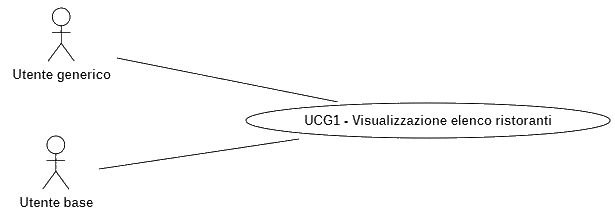
\includegraphics[width=0.8\textwidth]{./uml/UCG1.png} 
	\caption{Visualizzazione elenco ristoranti}
	\label{fig:UCG1}
  \end{figure}

\begin{itemize}
	\item \textbf{Attori principali:} 
	\begin{itemize}
		\item Utente generico.
		\item Utente base.
	\end{itemize}

	\item \textbf{Precondizione:}
	      L'utente è connesso al Sistema.

	\item \textbf{Postcondizione:} L'Attore principale visualizza una lista di
	      ristoranti. Di \textit{default} la lista viene presentata in ordine decrescente di valutazione.

	\item \textbf{Scenario principale:}
	      \begin{enumerate}

		      \item Il Sistema presenta all'Attore principale un elenco di ristoranti disposti in ordine decrescente di valutazione media;

		      \item L'Attore principale visualizza la lista dei ristoranti secondo tale visualizzazione.

	      \end{enumerate}
\end{itemize}
